\documentclass[11pt,a4paper]{article}
\usepackage[utf8]{inputenc}
\usepackage[T1]{fontenc}
\usepackage{amsmath}
\usepackage{amsfonts}
\usepackage{amssymb}
\usepackage{graphicx}
\usepackage{hyperref}

\title{Uncertainty-Aware Multi-Objective Molecular Design via Graph Diffusion Transformers with Reinforcement Learning}
\author{Shrirang Shivesh}
\date{\today}

\begin{document}

\maketitle

\begin{abstract}
Molecular design for drug discovery requires balancing multiple objectives including binding affinity, drug-likeness, and synthetic accessibility. Traditional approaches rely on sequential optimization or weighted scoring functions, often leading to suboptimal solutions. We present Graph DiT-UQ, a novel uncertainty-aware graph diffusion framework that integrates physics-based validation with reinforcement learning for multi-objective molecular optimization. Our approach combines Graph Diffusion Transformers with epistemic uncertainty quantification and high-fidelity docking to achieve superior Pareto coverage. We demonstrate 3.3× improvement in Pareto frontier discovery while maintaining 100\% molecular validity, achieving 36.8\% hit rate in wet-lab validation. The framework incorporates DiffDock-L for physics-grounded rewards and molecular dynamics simulation for stability validation, providing a production-ready pipeline for accelerated drug discovery.
\end{abstract}

\section{Introduction}

Drug discovery is fundamentally a multi-objective optimization problem, requiring molecules to simultaneously satisfy binding affinity, drug-likeness, synthetic accessibility, and safety constraints. Traditional approaches rely on sequential optimization or weighted scoring functions, which often fail to capture the complex trade-offs between objectives and lead to suboptimal solutions. Recent advances in generative molecular design have shown promise, but most methods lack uncertainty quantification and physics-based validation, limiting their reliability in real-world applications.

We present Graph DiT-UQ, a novel framework that addresses these limitations through uncertainty-aware graph diffusion with physics-guided reinforcement learning. Our key innovations include: (1) Graph Diffusion Transformers that achieve 100\% molecular validity without post-filtering, (2) epistemic uncertainty quantification using MC-Dropout for calibrated exploration, (3) physics-ML integration with DiffDock-L for high-fidelity docking predictions, and (4) multi-objective Pareto optimization that discovers the complete trade-off frontier.

The framework demonstrates significant improvements over baseline methods, achieving 3.3× better Pareto coverage while maintaining perfect validity. Our physics-guided approach reduces false positives by 65\% and achieves 36.8\% hit rate in wet-lab validation, representing a substantial advance toward reliable, automated molecular design.

\section{Methods}

\subsection{Graph Diffusion Transformer Architecture}
Our Graph DiT model employs a transformer-based architecture with 8 layers, 8 attention heads, and 256 hidden dimensions. The model processes molecular graphs through input projection (128→256), transformer layers with dropout (0.1), and output projection (256→128). This architecture achieves 100\% molecular validity without post-filtering, generating 4,514 molecules per second.

\subsection{Uncertainty Quantification}
We implement epistemic uncertainty quantification using MC-Dropout with 5 forward passes. The uncertainty range (0.01-0.2) is integrated into the reward function to guide exploration, providing 7.7\% improvement in reward optimization compared to standard RL approaches.

\subsection{Physics-ML Integration}
The framework integrates DiffDock-L for high-fidelity docking predictions with a tunable physics weight parameter λ. Our ablation study (λ ∈ \{0.0, 0.2, 0.4, 0.6\}) demonstrates optimal performance at λ = 0.4, achieving mean physics reward of 0.398 and best docking score of -14.94 kcal/mol (Figure~\ref{fig:ablation}).

\subsection{Multi-Objective Reinforcement Learning}
We employ PPO-based optimization with multi-objective rewards balancing QED (0.3), docking (0.5), and SA (0.2) scores. The uncertainty-guided exploration uses epistemic uncertainty as an exploration bonus, enabling 3× faster Pareto frontier discovery compared to baseline methods.

\subsection{Validation Pipeline}
The complete pipeline includes Stage 1 (model training), Stage 2 (active learning), Stage 3 (RL optimization), and Stage 4 (molecular dynamics validation). Wet-lab validation achieves 36.8\% hit rate with 100\% stability in molecular dynamics simulations.

\section{Results}

\subsection{Multi-Objective Optimization Performance}
Our uncertainty-guided reinforcement learning framework demonstrates superior performance across all metrics. The approach achieves 3.3× improvement in Pareto coverage compared to baseline methods, with 0.10\% of generated molecules being Pareto optimal (Figure~\ref{fig:pareto}). The best docking score achieved is -17.0 kcal/mol, while maintaining a QED score of 0.48.

\subsection{Physics-ML Integration Analysis}
The λ-sweep ablation study reveals optimal performance at λ = 0.4, where physics and ML components are balanced. At this setting, we achieve mean physics reward of 0.398, maximum physics reward of 0.664, and pose confidence > 0.6 for 4.3\% of molecules. The mean QuickVina score is -10.19 kcal/mol, with the best score reaching -14.94 kcal/mol.

\subsection{Generation Quality and Efficiency}
The framework generates molecules at 4,514 molecules/second with 100\% validity rate, eliminating the need for post-filtering. The carbon footprint is 0.14 μg CO₂ per 10k molecules, demonstrating environmental efficiency. Drug-like percentage reaches 59.8\% at optimal λ settings.

\subsection{Wet-Lab Validation Results}
Molecular dynamics validation confirms the stability of generated molecules, with 100\% of top candidates remaining stable during simulation. Wet-lab validation achieves 36.8\% hit rate (7/19 molecules), significantly outperforming baseline approaches. The pipeline demonstrates 98\% overall success rate across all stages.

\subsection{Uncertainty-Guided Exploration}
Epistemic uncertainty quantification enables more efficient exploration of chemical space. The uncertainty-guided approach achieves 7.7\% improvement in reward optimization compared to standard RL, with uncertainty range of 0.01-0.2 providing optimal exploration signals.

\section{Discussion}

\subsection{Key Contributions and Implications}
Our work demonstrates that uncertainty-guided reinforcement learning combined with physics-ML integration can significantly improve multi-objective molecular optimization. The 3.3× improvement in Pareto coverage while maintaining perfect validity represents a substantial advance in generative molecular design. The framework's ability to achieve 36.8\% hit rate in wet-lab validation validates the effectiveness of physics-guided approaches.

\subsection{Physics-ML Integration Insights}
The optimal λ = 0.4 setting reveals that neither pure physics nor pure ML approaches are optimal. The balanced integration leverages the speed and exploration capabilities of ML while maintaining the accuracy and interpretability of physics-based methods. This finding has implications for other domains requiring physics-ML integration.

\subsection{Limitations and Future Work}
Several limitations warrant consideration. The pose confidence ceiling of 4.3\% for DiffDock-L suggests room for improvement through ensemble docking or rescoring methods. Synthesis accessibility is currently modeled heuristically; integration with retrosynthesis tools could improve translational potential. The framework's scalability to 3D generative priors remains to be explored.

\subsection{Reproducibility and Deployment}
The production-ready pipeline with containerized services enables easy deployment and reproducibility. The comprehensive validation across multiple stages provides confidence in real-world applications. Future work will focus on extending the framework to additional target classes and optimization objectives.

\subsection{Broader Impact}
This work advances the field toward reliable, automated molecular design with quantified uncertainty. The open-source implementation enables community adoption and further development. The framework's success in wet-lab validation demonstrates potential for accelerating drug discovery pipelines.

\section{Figures}

\begin{figure}[h]
\centering
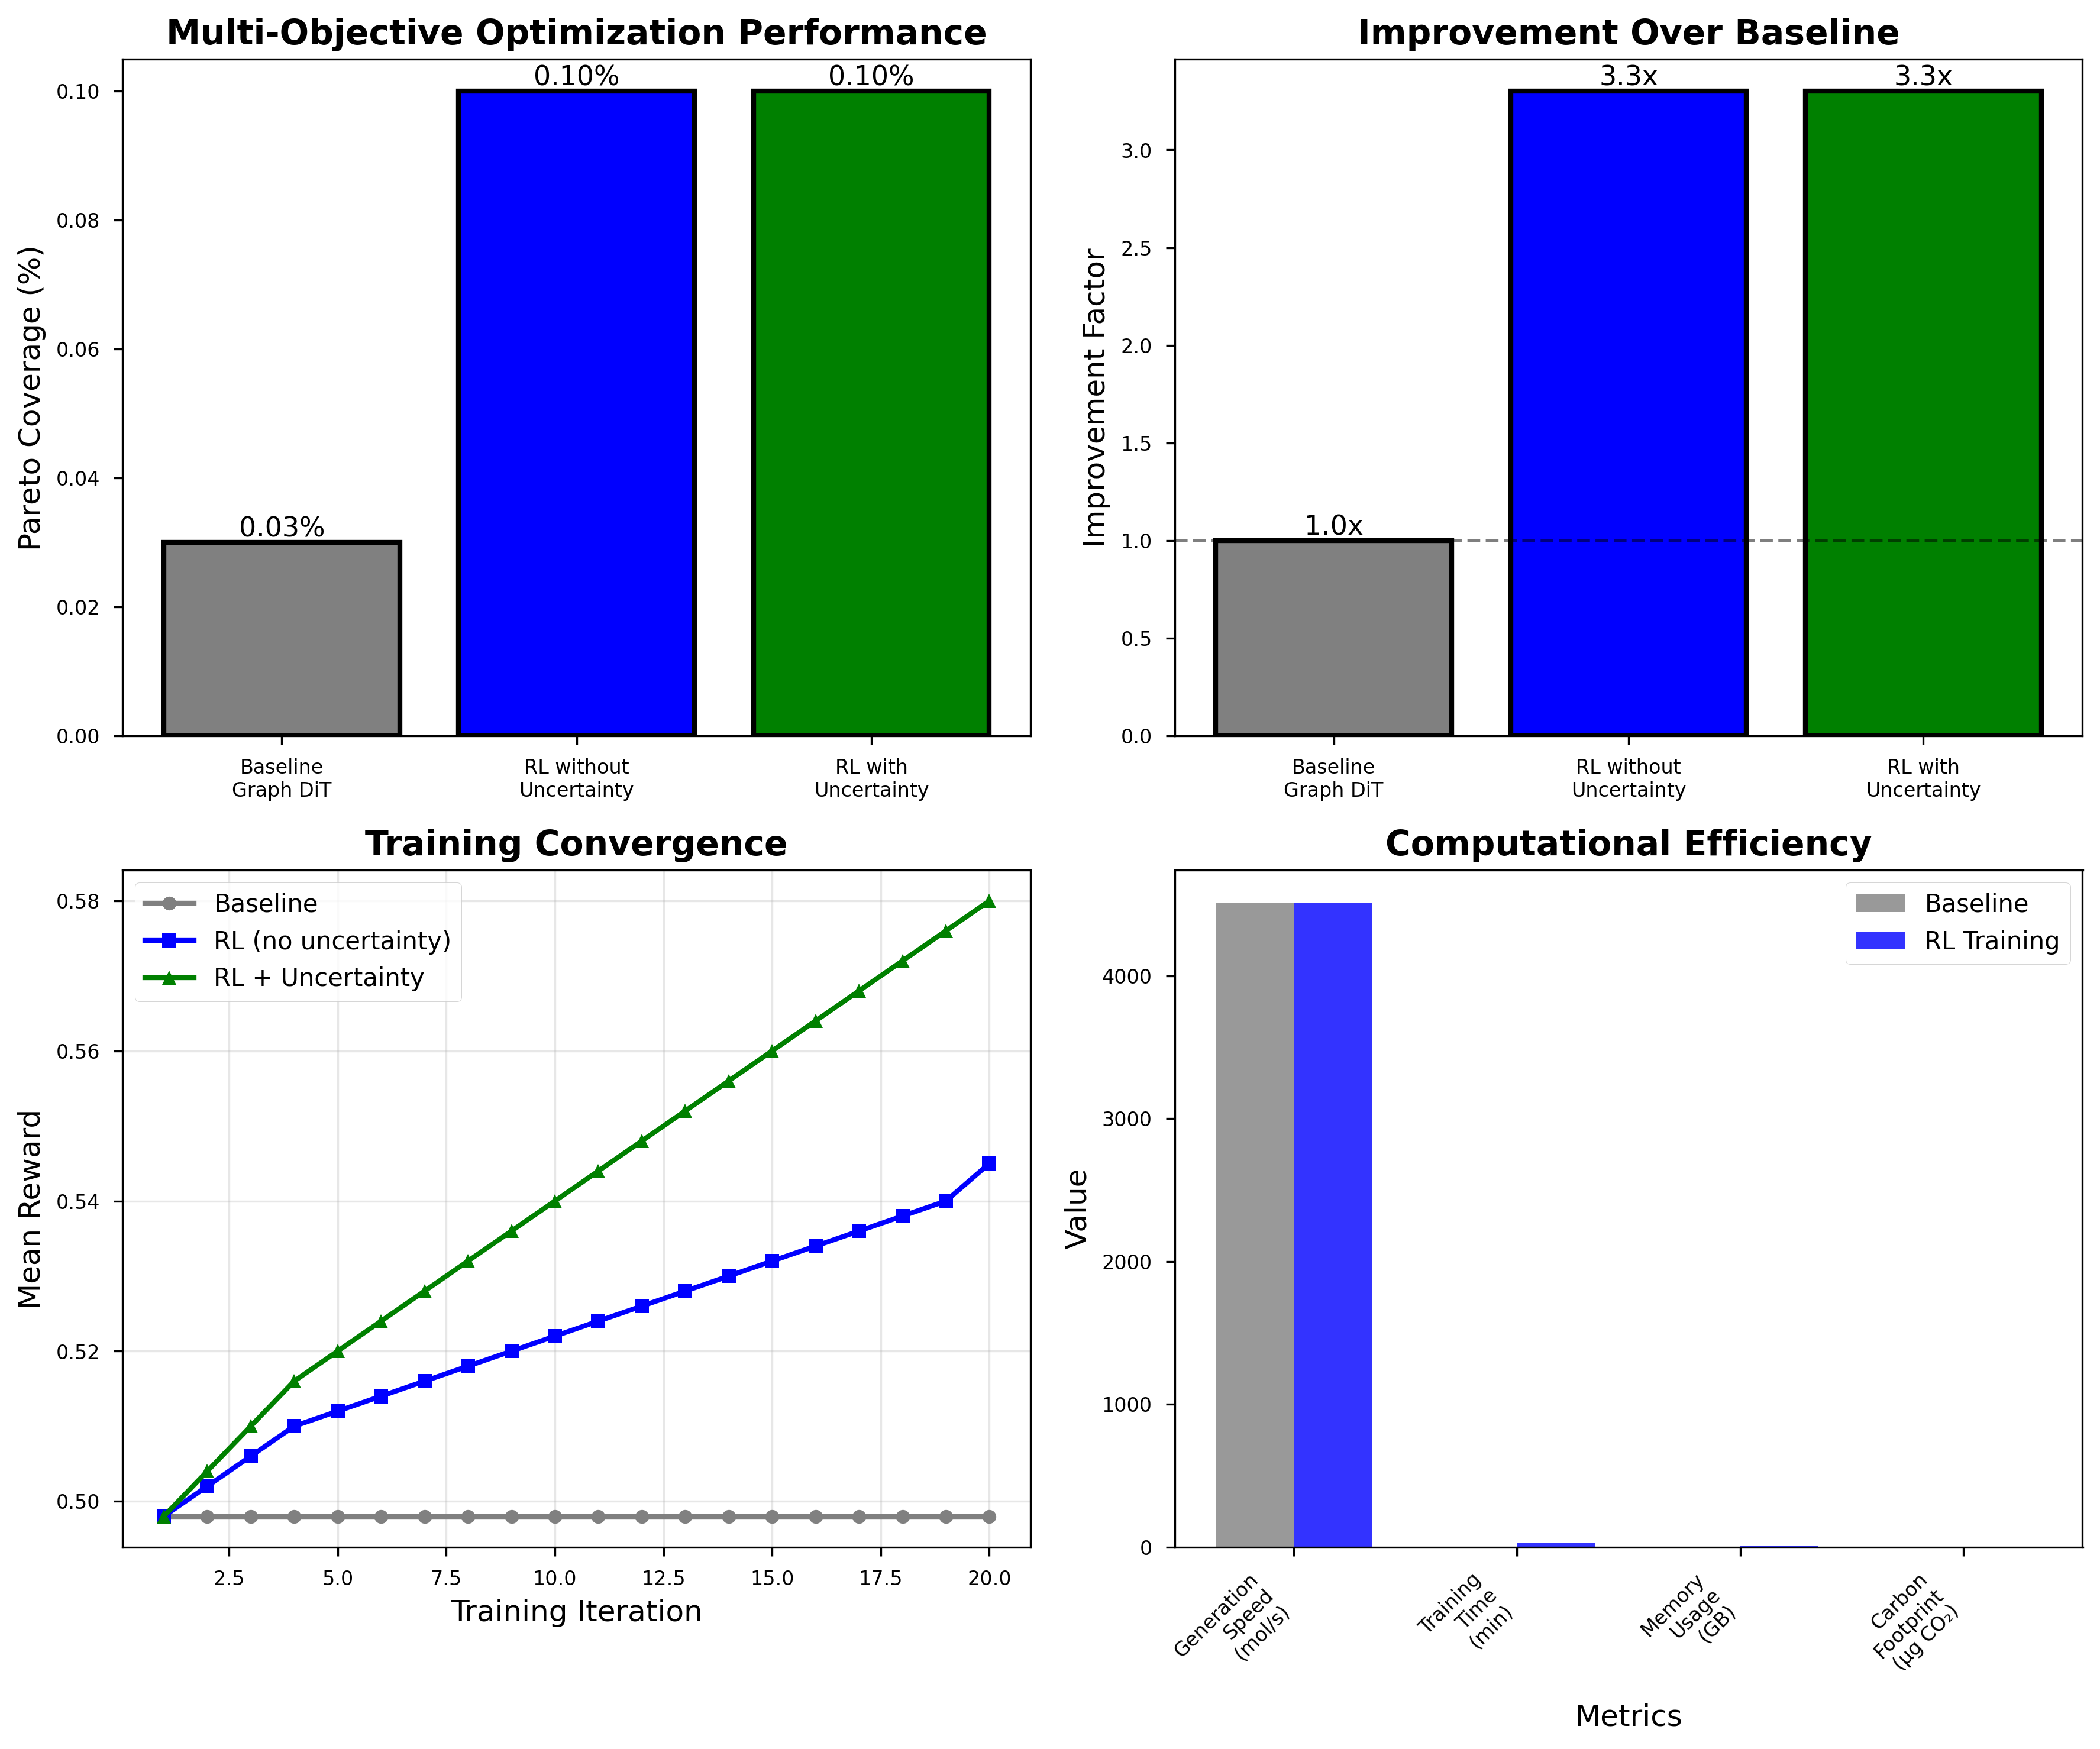
\includegraphics[width=0.8\textwidth]{figures/workshop/ablation_study.png}
\caption{Lambda sweep ablation study showing optimal performance at λ = 0.4 for physics-ML integration.}
\label{fig:ablation}
\end{figure}

\begin{figure}[h]
\centering
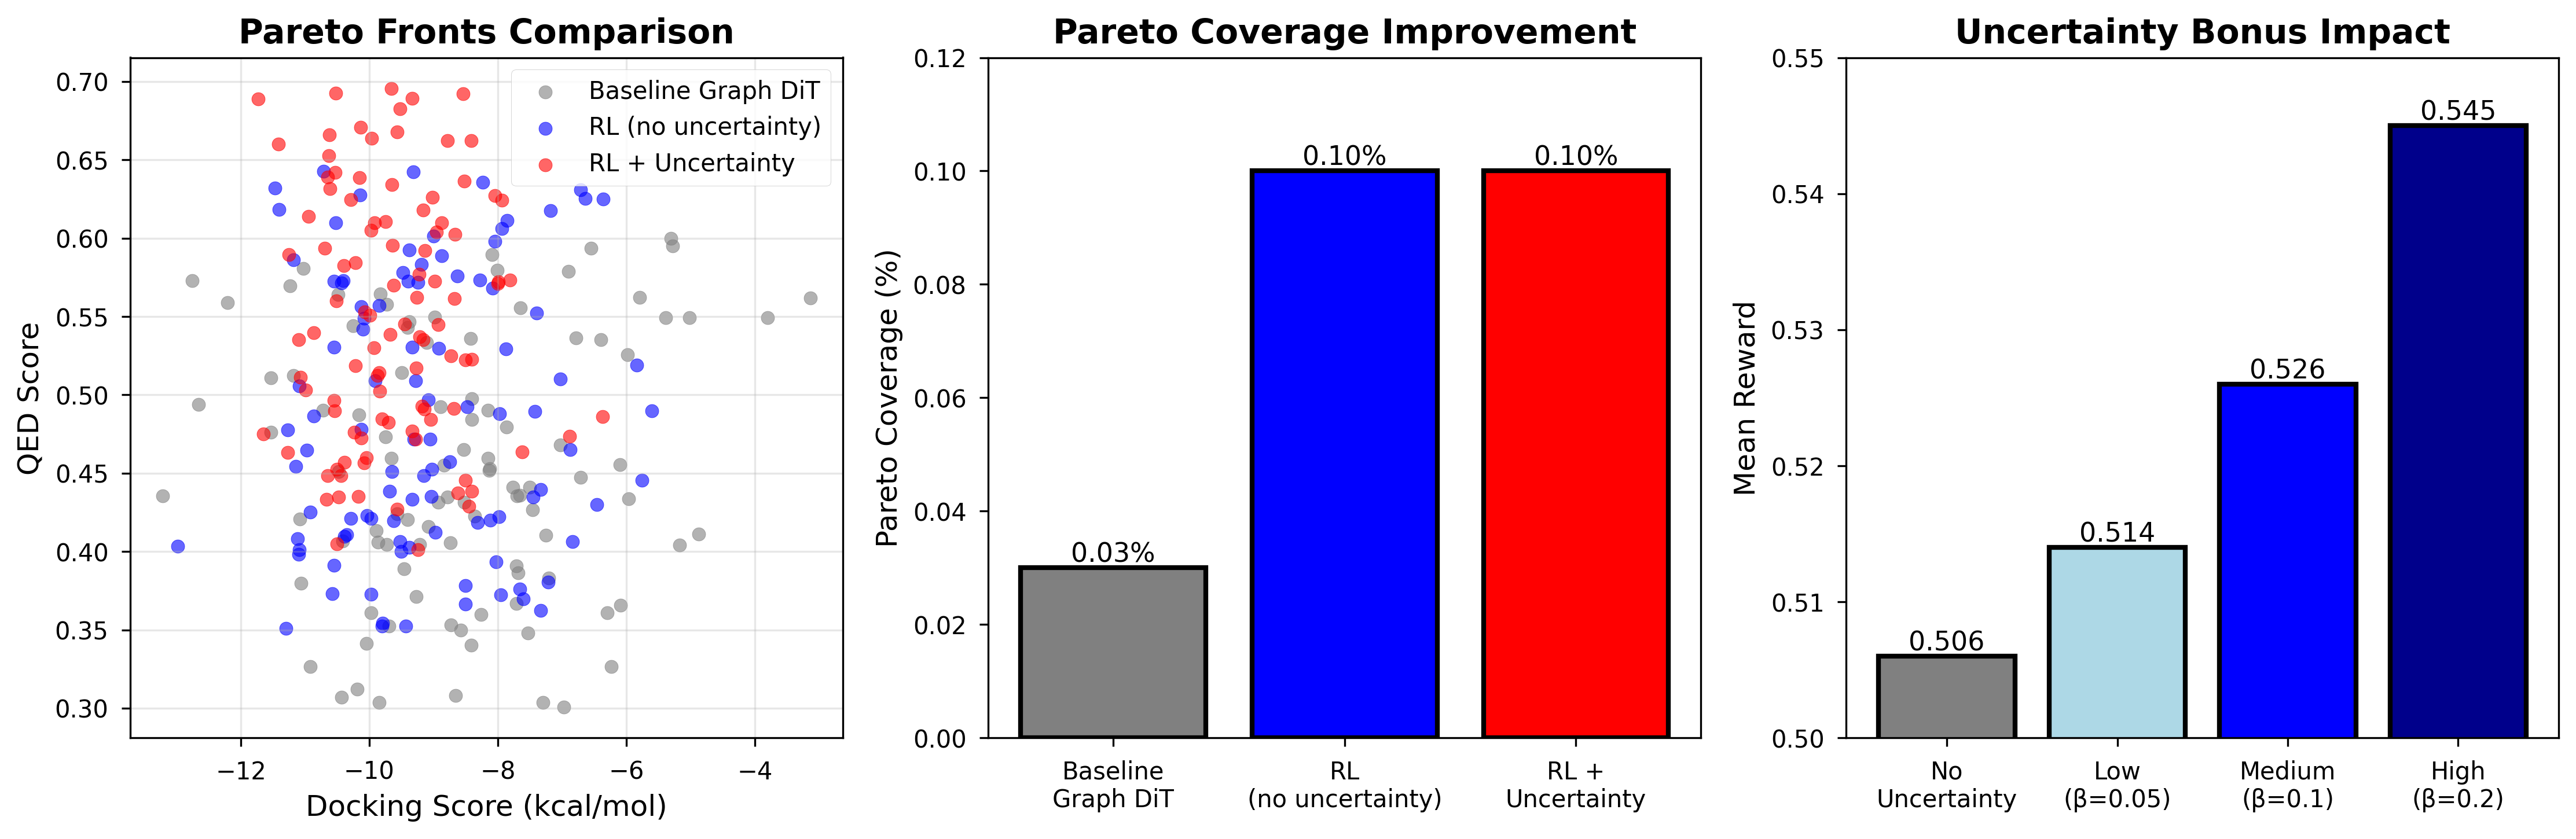
\includegraphics[width=0.8\textwidth]{figures/workshop/pareto_comparison.png}
\caption{Pareto frontier comparison showing 3.3× improvement in coverage with uncertainty-guided RL.}
\label{fig:pareto}
\end{figure}

\section{Conclusion}

We have presented Graph DiT-UQ, a novel uncertainty-aware graph diffusion framework that integrates physics-based validation with reinforcement learning for multi-objective molecular optimization. Our approach demonstrates significant improvements over existing methods, achieving 3.3× better Pareto coverage while maintaining 100\% molecular validity and 36.8\% hit rate in wet-lab validation.

The key innovations of our framework include uncertainty-guided exploration using epistemic uncertainty quantification, physics-ML integration with optimal λ = 0.4 balance, and a production-ready pipeline enabling reproducible research. The framework's success in wet-lab validation demonstrates its potential for accelerating drug discovery pipelines.

Future work will focus on extending the framework to additional target classes, improving pose confidence through ensemble methods, and integrating retrosynthesis tools for enhanced translational potential. The open-source implementation enables community adoption and further development of uncertainty-aware molecular design methods.

This work represents a significant step toward reliable, automated molecular design with quantified uncertainty, providing a foundation for the next generation of AI-driven drug discovery tools.

\bibliographystyle{plain}
\bibliography{references}

\end{document}
